\documentclass{article}
\usepackage{mainPoly}

\title{Dérivation}
\author{Première Spécialité Mathématiques}
\date{}

\begin{document}
\maketitle
\section{Taux de variation}
\begin{tcolorbox}
\begin{definition}
Soit $f$ une fonction définie sur un intervalle $I$. On prend $a < b \in I$. On appelle \textbf{taux de variation de $f$ entre $a$ et $b$} la grandeur
\begin{equation*}
\dfrac{f(b)-f(a)}{b-a}
\end{equation*}
\end{definition}
\end{tcolorbox}
\begin{example}
Une voiture roule pendant une heure. Soit $f(t)$ la distance parcourue en \unit{\kilo\meter} en fonction du temps $t$ en \unit{\minute}.
\begin{enumquestions}
\item Quelle est l'intervalle de définition de $f$ ? \answersline
\item Dessiner sur le repère suivant une courbe représentative possible pour $f$.
\begin{center}
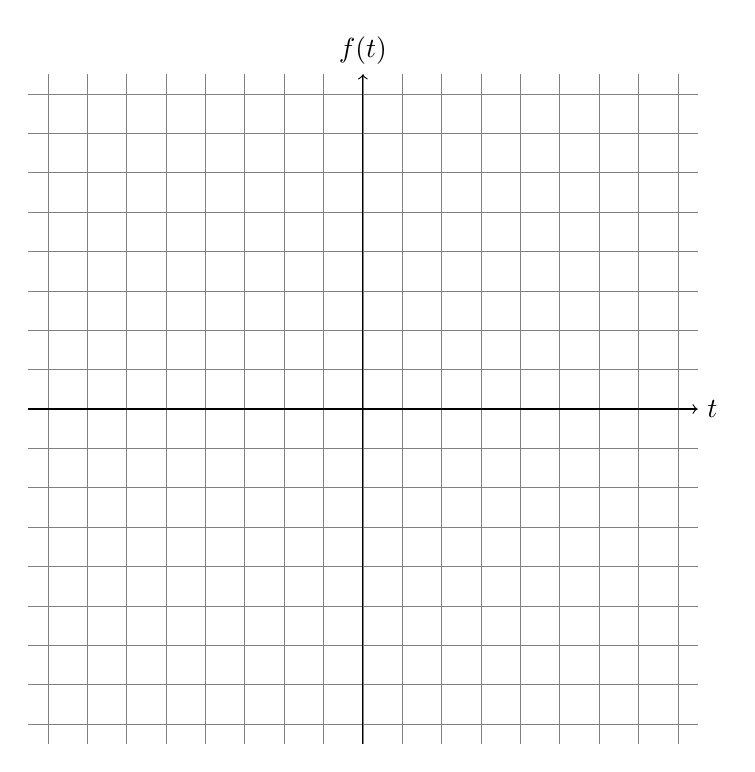
\begin{tikzpicture}
\draw[help lines] (-4.25,-4.25) grid[step=0.5] (4.25,4.25);
\draw[->] (-4.25,0) -- (4.25,0) node[right] {$t$};
\draw[->] (0,-4.25) -- (0,4.25) node[above] {$f(t)$};
\end{tikzpicture}
\end{center}
\item En fonction de votre réponse, donner le taux de variation de $f$ entre $0$ et $30$, et entre $30$ et $60$.
\vspace*{0.2cm}

\emptybox{2cm}
\item Comment interpréter votre résultat ? \answersline
\end{enumquestions}
\end{example}
\newpage
\begin{tcolorbox}
\begin{proposition}
Soit $f$ un fonction définie sur un intervalle $I$, et $a < b \in I$. Si on se place sur un repère orthonormé, et que l'on considère les points $A(a;f(a))$ et $B(b;f(b))$, alors le taux de variation de $f$ entre $a$ et $b$ correspond à la pente de la droite entre $A$ et $B$. 
\end{proposition}
\end{tcolorbox}
\begin{center}
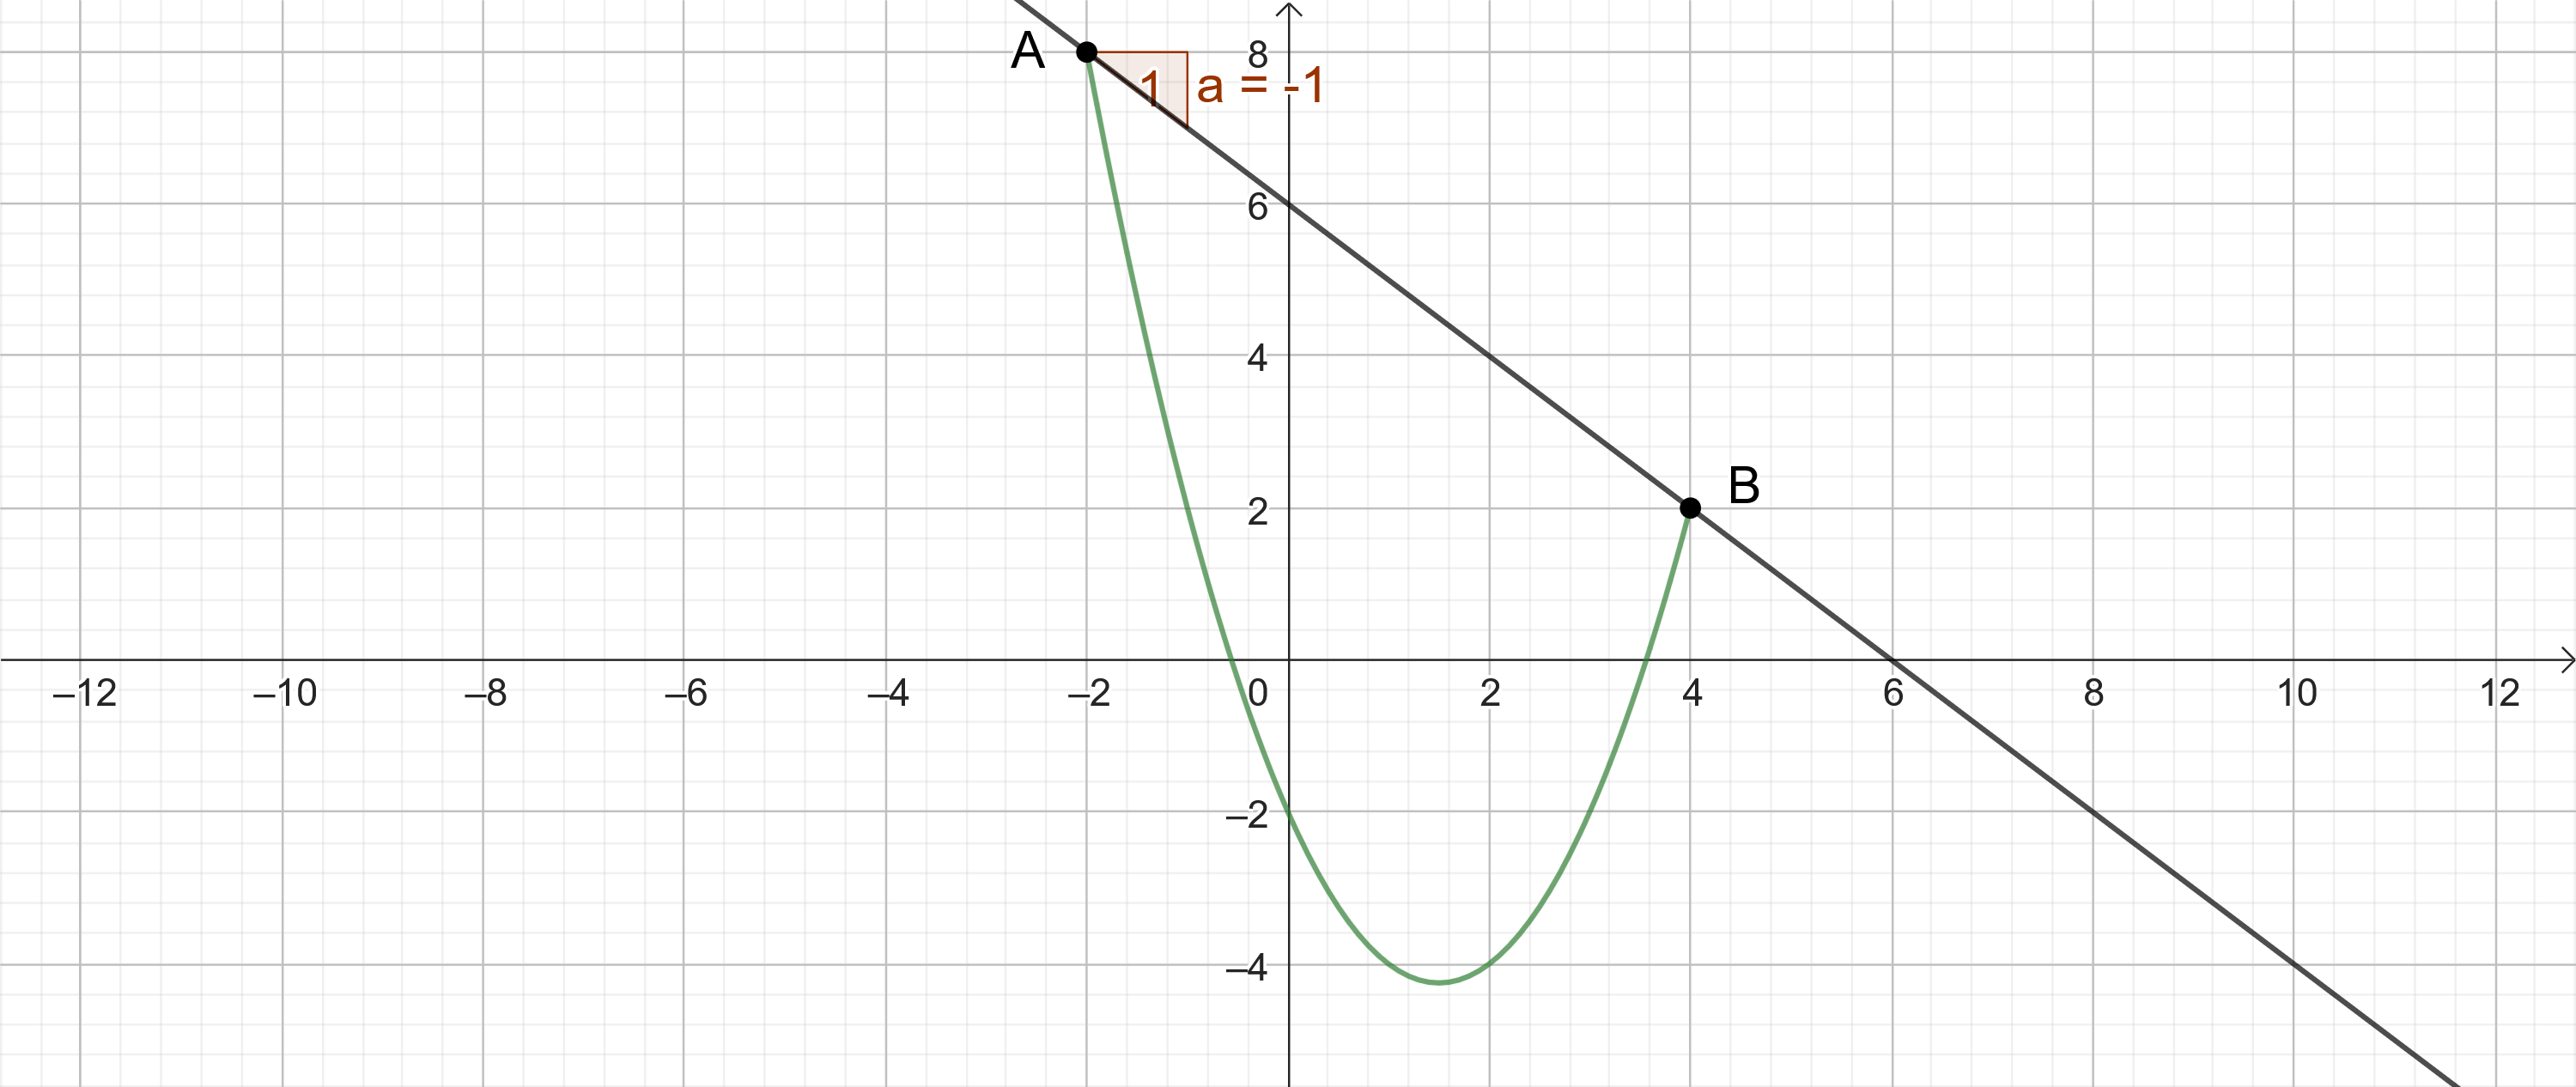
\includegraphics[width=\textwidth]{Taux_variation_pente.png}
\end{center}
\begin{remark}
Le taux de variation d'une fonction entre $a$ et $b$ répond à la question suivante : \textbf{Pour chaque abscisse parcourus entre $a$ et $b$, de combien d'ordonnées sommes-nous montés ou descendus ?}
\end{remark}
\begin{tcolorbox}
\begin{proposition}
Soit $f$ une fonction définie sur un intervalle $I$. Soit $J \subseteq I$ un intervalle.
\begin{itemize}
\item Si $f$ est croissante sur $J$, alors pour tout $a < b \in J$, le taux de variation de $f$ entre $a$ et $b$ est positif.  
\item Si $f$ est décroissante sur $J$, alors pour tout $a < b \in J$, le taux de variation de $f$ entre $a$ et $b$ est négatif.  
\end{itemize}
\end{proposition}
\end{tcolorbox}
\begin{remark}
\textbf{Les réciproques sont fausses :} un taux de variation de $f$ entre $a$ et $b$ positif n'implique pas que la fonction $f$ est croissante sur l'intervalle $[a;b]$.
\end{remark}
\begin{example}
Soit $f \colon x \mapsto (x-1)^2 - 2$ définie sur $[-2;3]$.
\begin{enumquestions}
\item Donner un intervalle $I$ sur lequel $f$ est croissante, et un intervalle $J$ sur lequel $f$ est décroissante : 

$I =$ \answersline; $J = $ \answersline
\item Choisir deux valeurs dans chacun des intervalles, et calculer les taux de variations de $f$ entre ces deux valeurs.

\answersline
\item Calculer le taux de variation entre $-2$ et $2$. Que peut-on en déduire ? \answersline
\end{enumquestions} 
\end{example}
\end{document}